\documentclass[sigconf,nonacm,11pt]{acmart}

\usepackage{graphicx}
\usepackage{booktabs}
\usepackage{xcolor}
\usepackage{microtype}

% Strip ACM-specific copyright / CCS / reference machinery
\setcopyright{none}
\settopmatter{printacmref=false, printccs=false, printfolios=true}
\renewcommand\footnotetextcopyrightpermission[1]{}
\pagestyle{plain}

\acmConference[ECE 284]{ECE 284 Final Project Report}{Spring 2026}{University of California, San Diego}
\acmYear{2026}
\acmISBN{}
\acmDOI{}
\acmPrice{}

\title{Can a Large Language Model Choose Better Signal-Processing Parameters? A Controlled Benchmark of LLM-Generated $\lambda$ for Motion-Robust PPG Heart-Rate Estimation}

\author{Javen Cao}
\affiliation{%
  \institution{University of California, San Diego}
  \city{La Jolla}
  \state{California}
  \country{USA}
}
\email{jacao@ucsd.edu}

\renewcommand{\shortauthors}{J. Cao}

\begin{document}

\begin{abstract}
Photoplethysmography (PPG) heart-rate (HR) estimation on wrist-worn devices is severely degraded by motion artifacts. A classical remedy, accelerometer-informed spectral subtraction, depends on a weight $\lambda$ that controls how aggressively motion energy is removed; in practice $\lambda$ is fixed, even though the optimal value varies window to window. We ask whether a large language model (LLM) can act as a \emph{per-window parameter generator}, reading interpretable spectral features and emitting a suitable $\lambda$. We build a controlled benchmark on the IEEE SPC 2015 dataset (11 subjects, leave-one-subject-out) comparing four $\lambda$-selection policies under an identical signal-processing pipeline---fixed $\lambda$, a supervised Random-Forest $\lambda$ regressor (RF-$\lambda$), an LLM $\lambda$ generator (LLM-$\lambda$), and a ground-truth oracle---plus an external Random-Forest HR predictor (RF-HR) as a different modeling paradigm. LLM-$\lambda$ recovers 28\% of the oracle's $\lambda$-headroom, roughly three times the recovery of RF-$\lambda$ (8\%), and is the numerically strongest method in low-motion windows. However, the oracle improves fixed $\lambda$ by only 3.63\,BPM, and high-motion windows remain dominated by RF-HR. We conclude that LLM-as-parameter-generator is a feasible paradigm whose value is bounded by the limited leverage of $\lambda$ and by the spectral-subtraction architecture it controls, rather than by $\lambda$-decision quality alone.
\end{abstract}

\maketitle

\section{Motivation}

Wrist-worn PPG sensors are now the dominant consumer modality for continuous heart-rate monitoring, appearing in nearly every smartwatch and fitness band. PPG works by shining light into the skin and measuring the small fluctuations in reflected light caused by blood-volume changes with each heartbeat. The method is cheap, comfortable, and non-invasive---but it has a well-known failure mode: \textbf{motion}. When the wrist moves, the pressure between sensor and skin changes and the optical path shifts, producing fluctuations that have nothing to do with the heartbeat. During exercise these motion artifacts can be larger than the cardiac signal itself, which is precisely when accurate HR matters most.

A standard signal-processing remedy uses a second sensor already present on the device: the accelerometer. Because the accelerometer measures wrist motion directly (and contains no cardiac information), its spectrum provides an imperfect but useful template of the motion artifact. \emph{Spectral subtraction} removes the motion component from the PPG spectrum by subtracting a scaled copy of the accelerometer spectrum. The scaling weight, $\lambda$, controls how much is removed. Setting $\lambda$ too low leaves motion artifacts in place; setting it too high erases the heartbeat along with the motion.

The difficulty is that the \emph{right} $\lambda$ is not constant. A subject sitting still needs almost no subtraction; a subject sprinting needs aggressive subtraction; and the coupling between accelerometer motion and PPG corruption varies between people and activities. The conventional approach simply fixes $\lambda$ to a single value, sacrificing this per-window adaptivity.

This project explores a different idea. Rather than using a large language model (LLM) as an end-to-end black box that predicts heart rate directly---a role in which it is hard to tell whether the model is reasoning or guessing---we place the LLM in a \textbf{narrow, controlled, and interpretable position}: looking at a compact summary of each window's spectral features and emitting a single parameter, $\lambda$. This framing turns a vague question (``can LLMs do HR estimation?'') into a precise one: \emph{can an LLM choose a better signal-processing parameter, per window, than a fixed value or a trained regressor?}

\section{Related Work}

\textbf{Classical spectral-processing methods.} The most direct ancestor of this work is TROIKA~\cite{TROIKA}, which combines signal decomposition, sparse spectral reconstruction, and accelerometer-informed spectral subtraction to estimate HR from motion-corrupted PPG, reporting an average error of 2.34\,BPM on the IEEE SPC 2015 dataset. A closely related method, JOSS~\cite{JOSS}, uses joint sparse spectrum reconstruction across PPG and accelerometer channels. These methods establish that classical signal processing can recover HR under motion, but at the cost of considerable algorithmic machinery (sparse solvers, harmonic tracking, multi-channel fusion).

\textbf{LLMs for physiological signals.} Recent work has begun to apply LLMs to wearable biosignal tasks. Feli et al.~\cite{Feli2025} propose an LLM-powered agent for PPG-based HR estimation within an orchestration framework, where the LLM coordinates analysis steps. This is the closest prior work to ours and directly motivates our research question; however, it frames the LLM as an \emph{orchestrator} of a pipeline rather than as a \emph{parameter generator} within a fixed pipeline, and motion-heavy regimes remain under-evaluated. Beyond HR, LLMs have been explored for explainable stress recognition from PPG~\cite{Can2026} and for cuffless blood-pressure estimation from wearable biosignals~\cite{Liu2024}, indicating growing interest in LLMs as components of physiological-signal systems---but the specific question of LLM-generated signal-processing parameters under heavy motion has not been systematically evaluated.

\textbf{LLMs as decision modules.} The broader idea of using LLMs to take actions or make structured decisions, rather than only generate text, is exemplified by ReAct~\cite{ReAct}, which interleaves reasoning and acting. This paradigm underpins the orchestration variant we leave to future work (Section~\ref{sec:conclusion}).

Direct prior work on using an LLM to generate spectral-subtraction parameters is, to our knowledge, limited; we therefore treat this as a controlled prototype rather than a comparison against an established method.

\section{Project Aim}

The central research question (RQ1) is:

\begin{quote}
\emph{Can an LLM-based parameter generator---producing a per-window $\lambda$ for spectral subtraction---improve over fixed and learned $\lambda$-selection baselines, and how close can it get to a supervised HR predictor?}
\end{quote}

To answer this cleanly, we adopt a \textbf{controlled-comparison} principle: every $\lambda$-selection policy runs inside an \emph{identical} signal-processing pipeline, so that the only variable is \textbf{how $\lambda$ is chosen}. This yields two distinct comparison axes:

\begin{enumerate}
\item \textbf{$\lambda$-policy axis (controlled):} fixed $\lambda$ vs.\ supervised RF-$\lambda$ vs.\ LLM-$\lambda$ vs.\ oracle $\lambda$. All four share the same bandpass $\to$ FFT $\to$ coupling-normalized spectral subtraction $\to$ HR-tracking pipeline. Differences are attributable solely to the $\lambda$ policy.

\item \textbf{Paradigm axis (reference):} the $\lambda$-controlled signal-processing family vs.\ an external Random-Forest HR predictor (RF-HR) that bypasses spectral subtraction entirely and learns a direct feature$\to$HR mapping. RF-HR has no $\lambda$; it is included as a reference point for whether parameter-tuned signal processing can compete with a conventional supervised-learning paradigm.
\end{enumerate}

A stretch question (RQ2)---whether an LLM \emph{orchestrator} (selecting and sequencing processing steps) outperforms the \emph{parametric} paradigm---was scoped as optional and is deferred to future work; this report focuses on a thorough evaluation of the parametric paradigm.

\section{Methodology}

\subsection{Dataset and Evaluation Protocol}

We use the IEEE Signal Processing Cup 2015 dataset of treadmill PPG with simultaneous ECG, sampled at 125\,Hz. Each recording provides one PPG channel, three-axis accelerometer data, and ECG-derived HR ground truth (in BPM). HR is estimated on 8-second windows with a 2-second shift between consecutive windows.

We obtained the data from a public mirror that contains 11 of the 12 subjects (subject 09 is absent from the mirror); subjects 01 and 04 use the TYPE01 (lower-intensity, up to 15\,km/h) protocol and the remaining subjects use TYPE02 (higher-intensity, up to 20\,km/h). All evaluation uses \textbf{leave-one-subject-out (LOSO)} cross-validation: trained methods are fit on the other 10 subjects and tested on the held-out subject. LOSO is the appropriate protocol here because random window splits would leak temporally adjacent windows of the same subject into both train and test, inflating performance. The error metric is mean absolute error (MAE) in BPM between the estimated HR and the ECG ground truth.

\subsection{Method A --- TROIKA-lite (fixed $\lambda$)}

Method A is a simplified reimplementation of the TROIKA spectral-subtraction pipeline, serving as the shared backbone for all $\lambda$-policy methods:

\begin{enumerate}
\item \textbf{Bandpass filter} the PPG (0.4--5\,Hz, 4th-order Butterworth, applied with zero-phase \texttt{filtfilt}). The 0.4--5\,Hz band corresponds to physiologically plausible HR (24--300\,BPM); zero-phase filtering avoids the peak-shifting that a causal filter would introduce.
\item \textbf{FFT} via periodogram (nfft\,=\,4096), giving the power spectral density (PSD).
\item \textbf{Coupling-normalized spectral subtraction} (detailed below).
\item \textbf{Peak selection with HR tracking} (detailed below).
\end{enumerate}

\textbf{Coupling normalization.} A diagnostic on the raw pipeline revealed that the PPG PSD and accelerometer PSD differ in magnitude by roughly three orders of magnitude (PPG~$\approx$~5000, accelerometer~$\approx$~3). With the na\"ive formula $\text{cleaned} = \text{PPG} - \lambda \cdot \text{accel}$, a value of $\lambda = 1.0$ subtracts almost nothing---spectral subtraction becomes a no-op. To make $\lambda$ meaningful, we estimate a coupling coefficient by least-squares regression of the PPG PSD onto the accelerometer PSD within the HR band, and subtract a scaled copy:

\begin{equation}
\text{cleaned} = \max\!\bigl(\text{PPG}_{\text{psd}} - \lambda \cdot \text{coef} \cdot \text{accel}_{\text{psd}},\ 0\bigr)
\end{equation}

where coef rescales the accelerometer spectrum to the PPG magnitude. This single change lowered subject-01 MAE from 24.6 to 20.9\,BPM and made $\lambda \in [0.1, 3.0]$ a meaningful operating range.

\textbf{HR tracking with cold start and self-correction.} After subtraction, the cleaned HR-band spectrum often contains several peaks of similar power (cardiac fundamental, cardiac harmonics, residual motion), and na\"ive maximum-peak selection jitters by $\pm$10--20\,BPM between adjacent windows. We constrain the current window's peak to lie within $\pm$15\,BPM of the previous window's HR estimate. To avoid locking onto an early error, the first 10 windows (cold start) ignore this constraint and use the global maximum; and if the strongest peak inside the tracking band is weaker than 50\% of the global maximum (self-correction threshold), the method falls back to the global maximum. Initial tracking (cold-start $N = 5$) improved subject-01 MAE to 13.6\,BPM, and the final configuration ($N = 10$) carries this gain forward.

\textbf{Deliberate simplifications.} Relative to full TROIKA, we omit M-FOCUSS sparse reconstruction and dual-channel fusion (we use one PPG channel). This is intentional: the goal is a controlled comparison of $\lambda$ policies, not a reproduction of TROIKA's absolute accuracy. The consequence is a substantially higher absolute error (15.07\,BPM overall vs.\ TROIKA's reported 2.34\,BPM). As the oracle analysis (Section~\ref{sec:results}) shows, even an optimal $\lambda$ cannot close this gap---the residual error is bound by the simplified architecture, not by $\lambda$ selection. We return to this point in the Discussion as one of the project's main findings, rather than treat it as a hidden weakness.

Final parameters: cold-start $N = 10$, self-correction threshold $T = 0.5$, tracking band $J = \pm 15$\,BPM, $\lambda = 1.0$. (All four $\lambda$-policy methods---Method A, LLM-$\lambda$, RF-$\lambda$, and the oracle---use this same $J = \pm 15$\,BPM tracking configuration, ensuring the pipeline is identical across the $\lambda$-policy axis.)

\subsection{Method B --- Random Forest HR predictor (RF-HR)}

Method B is a conventional supervised baseline on a different paradigm axis: it predicts HR directly from features, without spectral subtraction or any $\lambda$. For each window we extract 11 frequency-domain features: PPG dominant frequency, dominant power, HR-band energy, and peak-to-band ratio; accelerometer dominant frequency, dominant power, band energy, magnitude mean, and magnitude variance; and two cross features (PPG/accel peak ratio, frequency difference). A \texttt{RandomForestRegressor} (100 trees, fixed seed) is trained under LOSO. We do not tune hyperparameters: the goal is a simple, reproducible supervised baseline, not a maximally tuned model.

\subsection{Method C --- LLM $\lambda$ generator (LLM-$\lambda$)}

Method C is identical to Method A in every respect \emph{except} that $\lambda$ is generated per window by an LLM instead of fixed. For each non-cold-start window, we build a compact prompt containing: the top-3 PPG spectral peaks (frequency, power), the top-3 accelerometer peaks, the accelerometer intensity (magnitude variance), the coupling coefficient, the last three HR estimates, and the last three $\lambda$ values. The system prompt explains the meaning of $\lambda$ (under/over-subtraction) and asks for a single value in $[0.1, 3.0]$. The model returns strict JSON \texttt{\{"reasoning":~\ldots,~"lambda":~\ldots\}}; the returned $\lambda$ is fed into the \emph{same} spectral-subtraction and HR-tracking machinery as Method A.

We use DeepSeek-V4-flash, a cost-efficient, openly-priced instruction-tuned LLM, to keep evaluation cost low and reproducible; thinking mode is disabled and temperature is 0.3. (The original proposal specified Claude; we substituted DeepSeek for cost and latency reasons. The paradigm is model-agnostic, and cross-model generalization is left as a limitation.) A fallback harness guards reliability: API errors trigger up to two retries; malformed or schema-violating JSON falls back to $\lambda = 1.0$; out-of-range values are clamped; cold-start windows use $\lambda = 1.0$ without an LLM call. Across 1470 LLM calls in the full LOSO run, \textbf{zero fallbacks} were triggered.

\subsection{Oracle $\lambda$ and the $\lambda$-headroom metric}

To bound how much \emph{any} $\lambda$ policy could achieve within this architecture, we compute an oracle. For each non-cold-start window we sweep $\lambda$ over a grid (0.1 to 3.0, step 0.1), run the full pipeline including tracking, and select the $\lambda$ minimizing the absolute error against the ECG ground truth; ties are broken toward $\lambda = 1.0$. The oracle is \textbf{not deployable}---it requires the true HR---and it is a \emph{greedy per-window} oracle (the chosen $\lambda$ updates the tracking state for subsequent windows), so it is best read as a tight, architecture-constrained upper bound on $\lambda$ tuning rather than a global optimum.

We summarize how much of this bound each method captures with a single ratio:

\begin{equation}
\text{headroom recovery} \;=\; \frac{\text{MAE}_{\text{fixed}\lambda} - \text{MAE}_{\text{method}}}{\text{MAE}_{\text{fixed}\lambda} - \text{MAE}_{\text{oracle}}}
\end{equation}

\subsection{RF-$\lambda$ --- a supervised $\lambda$ regressor}

To test whether the LLM's contribution could be obtained more cheaply by a conventional model, we add RF-$\lambda$: a Random Forest (100 trees, fixed seed, LOSO) that takes the same 11 features as RF-HR but is trained to predict the \emph{oracle $\lambda$} of each window, rather than HR. Its predicted $\lambda$ (clamped to $[0.1, 3.0]$) is then fed into the identical Method-A pipeline. RF-$\lambda$ and LLM-$\lambda$ are comparable as $\lambda$-selection methods because both feed a predicted $\lambda$ into the same downstream pipeline; however, they are \textbf{not a perfectly input-matched comparison}: RF-$\lambda$ uses the 11 engineered tabular features, while LLM-$\lambda$ receives a richer prompt containing spectral-peak summaries and short HR/$\lambda$ history. We therefore interpret RF-$\lambda$ as a supervised $\lambda$-selection baseline, not as a controlled isolation of model class alone. There is no ground-truth leakage: the held-out subject's oracle labels are never used in training.

\section{Results}
\label{sec:results}

\subsection{$\lambda$-policy axis: fixed vs.\ RF-$\lambda$ vs.\ LLM-$\lambda$ vs.\ oracle}

\begin{figure}[t]
\centering
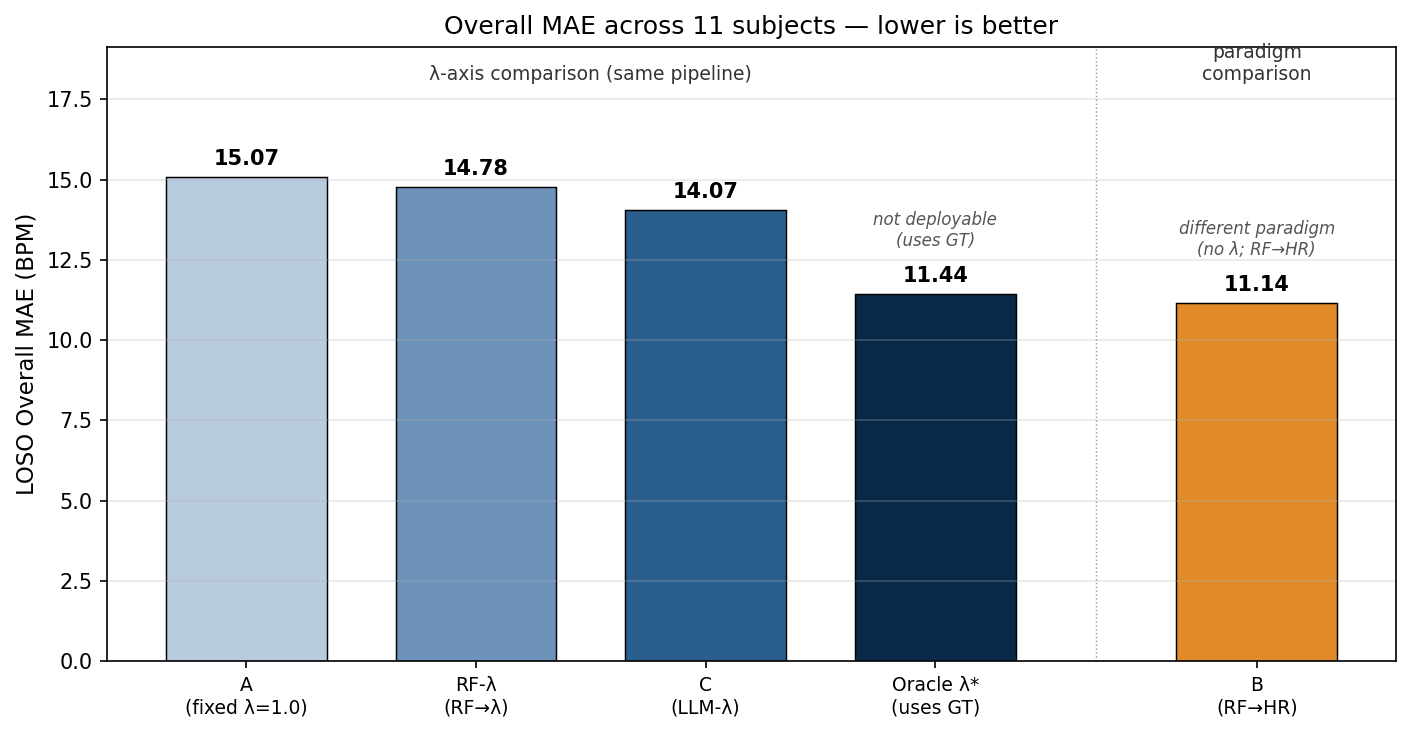
\includegraphics[width=\columnwidth]{figs/fig_overall_mae.png}
\caption{Overall LOSO MAE across five methods. Among $\lambda$-policy methods sharing the same pipeline (blue family), LLM-$\lambda$ is closest to the deployable best; the oracle bounds how far $\lambda$ tuning alone can take this architecture. Method B (RF-HR, orange) sits on a different paradigm axis and is the strongest deployable method on the full set.}
\label{fig:overall}
\end{figure}

Figure~\ref{fig:overall} accompanies this subsection. Under the identical pipeline, the four $\lambda$ policies give the overall LOSO MAE shown in Table~\ref{tab:lambda-policy} (lower is better).

\begin{table}[t]
\centering
\caption{$\lambda$-policy comparison under the identical Method-A pipeline ($J = \pm 15$, $N = 10$, $T = 0.5$).}
\label{tab:lambda-policy}
\small
\setlength{\tabcolsep}{4pt}
\begin{tabular}{@{}lrr@{}}
\toprule
$\lambda$ policy & MAE (BPM) & Recovery \\
\midrule
Fixed $\lambda = 1.0$ (A)       & 15.07 & 0\%    \\
RF-$\lambda$ (supervised)       & 14.78 & 8\%    \\
\textbf{LLM-$\lambda$ (C)}      & \textbf{14.07} & \textbf{28\%}   \\
Oracle $\lambda$ (upper bound)  & 11.44 & 100\%  \\
\bottomrule
\end{tabular}
\end{table}

Two observations stand out. First, \textbf{adaptive $\lambda$ helps but only modestly}: even the oracle improves fixed $\lambda$ by just 3.63\,BPM, showing that $\lambda$ is a limited control lever within this architecture. Second, \textbf{LLM-$\lambda$ recovers roughly three times more headroom than the supervised RF-$\lambda$} (28\% vs.\ 8\%, a 3.4$\times$ ratio). Inspecting the predicted $\lambda$ distributions explains why: RF-$\lambda$ collapses toward $\lambda \approx 1.0$ (std~$\approx$~0.11, range $[0.42, 1.70]$), effectively learning ``predict the mean'' from a label distribution dominated by ties at 1.0, whereas LLM-$\lambda$ spans most of $[0.1, 3.0]$ (observed range $[0.1, 2.9]$) and varies its output with motion state. In this specific $\lambda$-selection task and against this baseline, the LLM's prompt-conditioned prior was more effective than the trained tabular regressor.

\subsection{Paradigm axis: $\lambda$-controlled signal processing vs.\ RF-HR}

The external supervised HR predictor (RF-HR, Method B) achieves an overall MAE of \textbf{11.14\,BPM}, better than all $\lambda$-controlled methods on the full 11-subject set. RF-HR has no $\lambda$ and does not perform spectral subtraction; its advantage comes from learning a direct, nonlinear feature$\to$HR mapping that does not depend on correctly selecting a single spectral peak.

\textbf{Returning to RQ1:} LLM-$\lambda$ \emph{beats} the $\lambda$-decision baselines (fixed $\lambda$ and supervised RF-$\lambda$), but does \emph{not} match or beat RF-HR on the full 11-subject benchmark. In the outlier-excluded sensitivity analysis (Section~\ref{sec:outlier}), LLM-$\lambda$ nearly matches RF-HR, suggesting that much of the full-set gap is driven by an architecture-failure case rather than by broad underperformance across all subjects.

\subsection{Per-motion-level breakdown}

\begin{figure}[t]
\centering
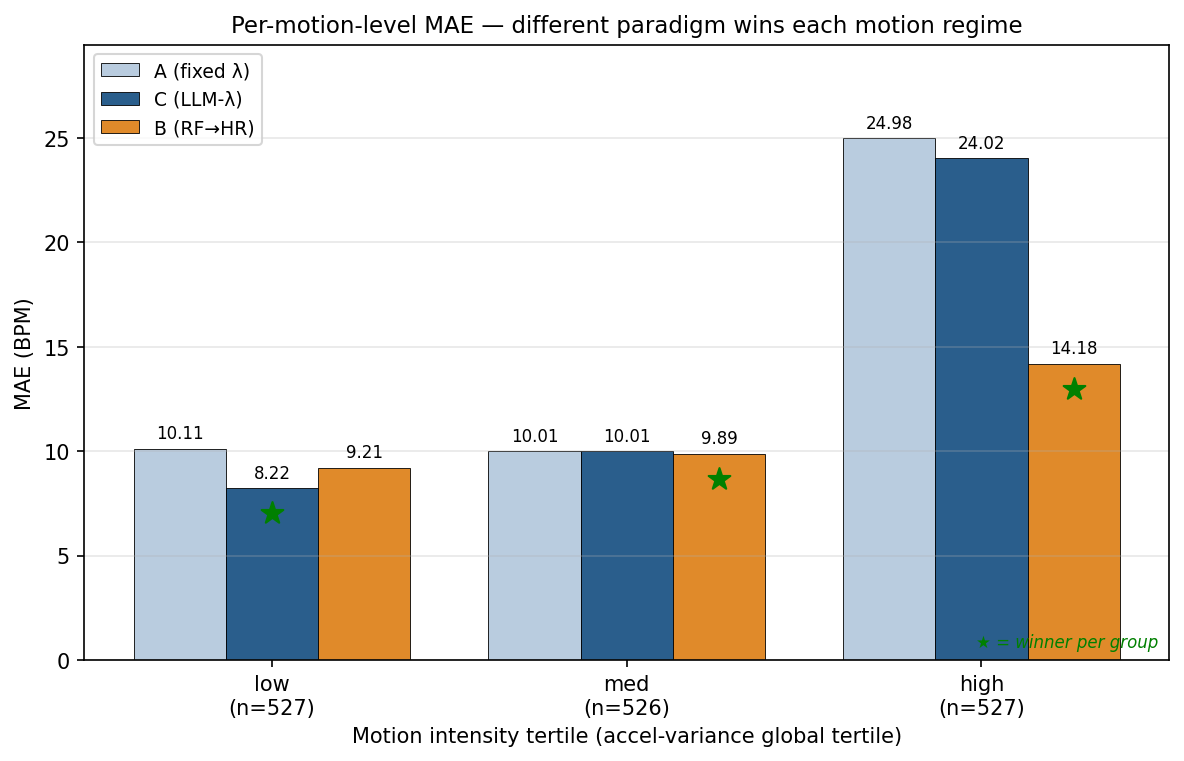
\includegraphics[width=\columnwidth]{figs/fig_motion_breakdown.png}
\caption{Per-motion-level MAE on the global tertile partition (low/med/high accelerometer variance, $n\!\approx\!527$ windows each). The winner of each tertile differs by method, and the gap is large at high motion: LLM-$\lambda$ leads at low motion, RF-HR carries high motion by $\sim$10\,BPM. No single method dominates everywhere.}
\label{fig:motion}
\end{figure}

Figure~\ref{fig:motion} accompanies this subsection. Pooling all 1580 windows and splitting them into low/medium/high motion tertiles by accelerometer magnitude variance gives the breakdown in Table~\ref{tab:motion}.

\begin{table}[t]
\centering
\caption{Per-motion-level MAE (BPM) across three deployable methods. Tertile partition is global (accel-variance percentiles 33.3\% / 66.7\%); $n \approx 527$ windows per tertile.}
\label{tab:motion}
\small
\setlength{\tabcolsep}{4pt}
\begin{tabular}{@{}lrrr@{}}
\toprule
            & low & med & high \\
\midrule
Method A (fixed $\lambda$) & 10.11           & 10.01           & 24.98 \\
Method B (RF-HR)           & 9.21            & 9.89            & \textbf{14.19} \\
Method C (LLM-$\lambda$)   & \textbf{8.22}   & 10.01           & 24.02 \\
\bottomrule
\end{tabular}
\end{table}

Performance is strongly \textbf{motion-dependent} in this benchmark. In \textbf{low-motion} windows, LLM-$\lambda$ is numerically the strongest method, ahead of RF-HR by about 1\,BPM---though we note this margin is within the range of expected noise and we did not compute confidence intervals. In \textbf{high-motion} windows, RF-HR is dramatically more robust, beating both spectral-subtraction methods by roughly 10\,BPM---a margin large enough to be a robust conclusion. The medium tertile is a near-tie. The high-motion result reflects the central failure of spectral subtraction: when motion energy dominates, no choice of $\lambda$ recovers the cardiac peak, and the tracking stage can lock onto the wrong frequency. This suggests that in high-motion regimes, feature-level supervised prediction may be more robust than peak-tracking after spectral subtraction.

\subsection{Outlier sensitivity and metric robustness}
\label{sec:outlier}

\begin{figure*}[t]
\centering
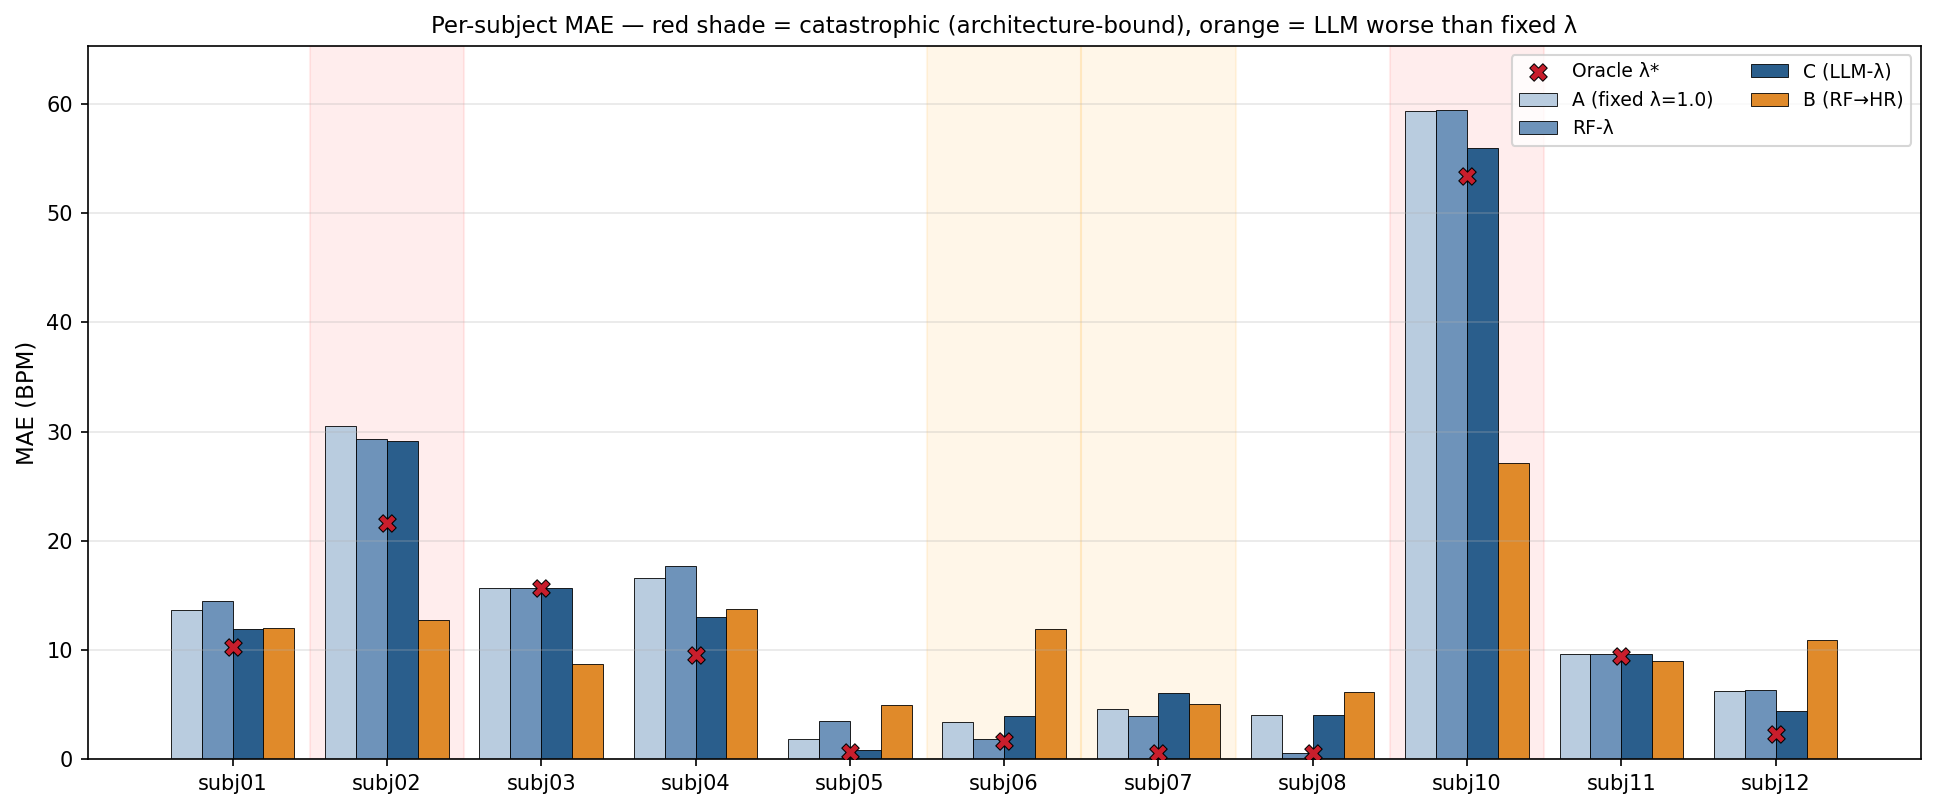
\includegraphics[width=0.94\textwidth]{figs/fig_per_subject_mae.png}
\caption{Per-subject MAE across the four deployable methods (bars) with oracle $\lambda$ overlaid as red $\times$ markers. Pink shading: catastrophic outliers (subj02/10) whose oracle MAE is also very high, indicating architecture-bound failure. Orange shading: subjects (subj06/07) where LLM-$\lambda$ is \emph{worse} than fixed $\lambda$---genuine LLM decision failures rather than architecture limits.}
\label{fig:persubj}
\end{figure*}

Figure~\ref{fig:persubj} accompanies this subsection. One subject (subj10) is a catastrophic, architecture-bound failure: even the oracle leaves 53.4\,BPM of error, indicating that no $\lambda$ recovers the correct HR. Because subj10 is shared by all spectral-subtraction-family methods, it inflates their overall (mean) MAE by $\sim$4.2--4.5\,BPM each, while it costs RF-HR only $\sim$1.6\,BPM, as shown in Table~\ref{tab:sensitivity}.

\begin{table}[t]
\centering
\caption{Sensitivity of overall MAE to a single architecture-failure subject (subj10). Excluding it reorders the methods and reveals that LLM-$\lambda$ nearly matches RF-HR.}
\label{tab:sensitivity}
\begin{tabular}{lrr}
\toprule
Method                & All 11 subjects & Excluding subj10 \\
\midrule
Oracle $\lambda$      & 11.44 & 7.25 \\
RF-HR (B)             & 11.14 & 9.54 \\
LLM-$\lambda$ (C)     & 14.07 & \textbf{9.88} \\
RF-$\lambda$          & 14.78 & 10.32 \\
Fixed $\lambda$ (A)   & 15.07 & 10.65 \\
\bottomrule
\end{tabular}
\end{table}

Excluding subj10, \textbf{LLM-$\lambda$ nearly matches RF-HR} (9.88 vs.\ 9.54, a 0.34\,BPM gap)---the overall-MAE gap between them is largely produced by a single architecture-failure case rather than by a broad performance difference. We report this as a sensitivity analysis supporting the main result, not as a replacement for it.

The mean is itself fragile here: across methods, median MAE (9.4--10.9\,BPM) is far lower than mean MAE, because two outlier subjects dominate the mean. RF-HR is the only method whose mean $\approx$ median (11.14 vs.\ 10.94), i.e., the only method without outlier-driven inflation.

\subsection{Per-subject $\lambda$ utilization and LLM failure modes}

\begin{figure*}[t]
\centering
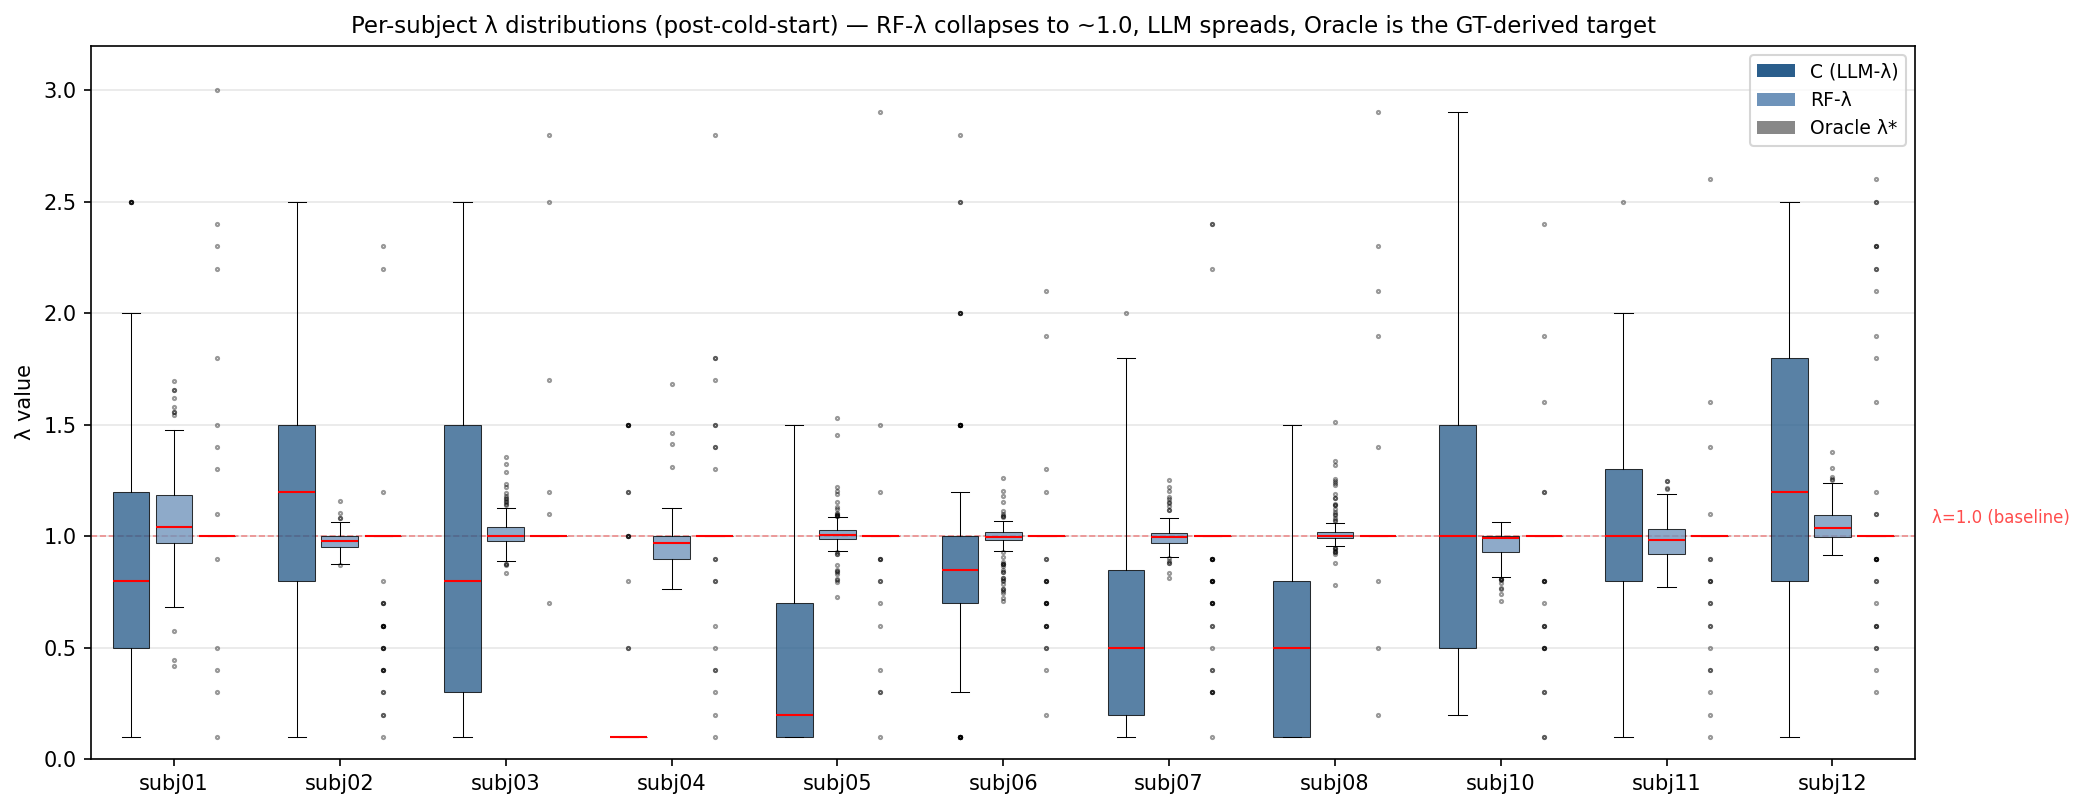
\includegraphics[width=0.94\textwidth]{figs/fig_lambda_distribution.png}
\caption{Per-subject post-cold-start $\lambda$ distributions for the three $\lambda$ sources. RF-$\lambda$ (middle box, blue-grey) collapses near 1.0 across all subjects; LLM-$\lambda$ (left, dark blue) spreads widely and adapts per subject; oracle $\lambda$ (right, grey) shows the GT-derived target. Red dashed line marks $\lambda = 1.0$.}
\label{fig:lambdadist}
\end{figure*}

Figure~\ref{fig:lambdadist} accompanies this subsection. Per-subject headroom recovery for LLM-$\lambda$ ranges widely. On most subjects it is positive (e.g., subj05 83\%, subj10 57\%, subj01 52\%), but on \textbf{subj06 and subj07 it is negative} ($-27\%$ and $-36\%$): here LLM-$\lambda$ is \emph{worse} than fixed $\lambda$. The two failure cases have different signatures. For subj07, the LLM assigned $\lambda < 0.5$ in roughly half of its windows, consistent with a ``low accelerometer intensity $\to$ low $\lambda$'' heuristic, whereas the oracle indicates $\lambda$ near 1.0 was optimal---a clear mis-weighting. For subj06 the signature is different: the LLM mostly chose mid-range $\lambda$ values that missed the oracle's preferred value by smaller margins. These are genuine LLM decision failures and may be addressable by prompt engineering, although this was not tested.

\section{Discussion}

\textbf{LLM-as-parameter-generator has real but bounded value.} The headline result is that a zero-shot LLM recovers roughly three times more $\lambda$-headroom than a supervised regressor trained on the same features (28\% vs.\ 8\%). That the LLM does this \emph{without any training labels}, while RF-$\lambda$---which \emph{is} trained on oracle labels---does worse, is the clearest evidence that LLM-$\lambda$ captures behavior this RF-$\lambda$ baseline did not extract under the current label distribution. The likely reason is partly a property of the labels themselves: the oracle $\lambda$ distribution is dominated by ties at 1.0, so a supervised regressor minimizing squared error is statistically pushed toward predicting the mean. The LLM, conditioned by its prior rather than fit to these labels, is freer to commit to larger deviations. We therefore frame the comparison carefully: in this specific task and against this specific baseline, the LLM's prompt-conditioned prior was more effective---not that LLMs are inherently better $\lambda$ choosers.

\textbf{But the lever is short.} The oracle improves fixed $\lambda$ by only 3.63\,BPM, so even a perfect per-window $\lambda$ policy cannot turn this pipeline into a competitive HR estimator. The main bottleneck is not primarily the quality of the $\lambda$ decision; it is the limited leverage of $\lambda$ together with the failure of spectral subtraction and tracking under heavy motion. subj10 makes this concrete: the oracle cannot fix it, so the failure is architectural, not parametric.

\textbf{Two failure sources coexist.} It would be too strong to say ``the bottleneck is the architecture, not the LLM's reasoning.'' The oracle bound shows that a large share of residual error is architecture-bound; \emph{simultaneously}, subj06/07 show that the LLM's own reasoning has a failure mode (the low-motion$\to$low-$\lambda$ heuristic mis-fires on subj07, and mid-range mis-selections on subj06). Both are real. Quantitatively, the architecture-driven failures (subj10/02) dominate the overall error, but the LLM's reasoning failures are not negligible and point to prompt engineering as a concrete improvement.

\textbf{Cost--value trade-off.} LLM-$\lambda$'s three-fold headroom advantage comes at a steep operational cost: a full LOSO run took $\sim$48 minutes ($\sim$2.0\,s per window) versus $\sim$3.5\,s for RF-$\lambda$---roughly 830$\times$ slower---and incurs API cost, whereas RF-$\lambda$ is essentially free once trained. For a deployed wrist device this matters: the LLM call is a cloud round-trip, not an on-device computation. RF-$\lambda$ is cheap and fast but learns a conservative policy from imperfect labels; LLM-$\lambda$ is expensive but exploits a prior the supervised model cannot. Neither is clearly preferable without specifying the deployment constraints.

\textbf{Method choice is motion-dependent.} The per-motion breakdown suggests that no single method is universally best: LLM-$\lambda$ leads in low motion, RF-HR is far more robust in high motion. A practical system might therefore benefit from motion-aware method switching---using the accelerometer to decide, per window, which estimator to trust.

\textbf{Reliability vs.\ correctness.} The harness was \emph{operationally} reliable---zero fallbacks across 1470 calls, with all JSON well-formed and in range. This is worth reporting for a system that places an LLM in the inner loop. But operational reliability is not decision reliability: valid, well-formed outputs (subj06/07) still degraded accuracy. The two should not be conflated.

\subsection*{Limitations}

\begin{itemize}
\item \textbf{Simplified architecture.} TROIKA-lite omits M-FOCUSS and dual-channel fusion; absolute MAE is $\sim$5$\times$ worse than full TROIKA. This is by design (to isolate $\lambda$) but limits external comparability.
\item \textbf{Mild tuning/evaluation overlap.} Pipeline design choices (coupling normalization, tracking parameters) were debugged on subject 01, which also appears in the LOSO evaluation. The internal A-vs-C comparison remains valid (same pipeline), but a fully blind protocol would tune only on training folds.
\item \textbf{RF-$\lambda$ is not input-matched to LLM-$\lambda$.} The two $\lambda$-selection methods see different input representations (engineered tabular features vs.\ a spectral-peak prompt), so the comparison reflects two complete $\lambda$-selection systems, not an isolation of model class alone.
\item \textbf{Single LLM backend and single run.} Results use one model (DeepSeek-V4-flash) at temperature 0.3, single seed; the LLM-$\lambda$ MAE is not averaged over multiple runs, and the A--C difference ($\sim$1\,BPM) is of the same order as plausible run-to-run noise. Cross-model generalization is untested.
\item \textbf{Imperfect oracle labels.} The oracle is a greedy, grid-limited, tie-broken-toward-1.0 per-window oracle; RF-$\lambda$ inherits these label imperfections.
\item \textbf{No statistical testing.} We report point estimates; confidence intervals and paired tests (especially for the $\sim$1\,BPM low-motion margin) are left as future analysis, as are subject-normalized motion tertiles and an explicit $\lambda$-vs-oracle decision-quality analysis.
\item \textbf{Incomplete dataset.} Subject 09 is missing from the mirror; 11 of 12 subjects are used.
\end{itemize}

\section{Conclusion}
\label{sec:conclusion}

This project asked whether an LLM can serve as a per-window parameter generator for spectral subtraction in motion-corrupted PPG heart-rate estimation. Using a controlled benchmark in which four $\lambda$-selection policies share an identical pipeline---plus an external supervised HR predictor as a paradigm reference---we found a nuanced answer. The LLM-generated $\lambda$ recovers 28\% of the oracle's $\lambda$-headroom, roughly three times that of a supervised $\lambda$ regressor trained on the same features, and is the numerically strongest method in low-motion windows. Yet the oracle shows the $\lambda$ lever is short (only 3.63\,BPM of total headroom), the supervised RF-HR predictor wins overall and dominates high-motion windows, and a single architecture-failure subject accounts for most of the gap between LLM-$\lambda$ and RF-HR.

The main takeaway is that \textbf{LLM-as-parameter-generator is a feasible and measurably useful paradigm, but its value is bounded by the architecture it controls---it is not solved by improving $\lambda$ decisions alone.} For severe PPG motion artifacts, the next bottleneck is not choosing $\lambda$ better; it is the spectral-subtraction-and-tracking architecture itself. Promising future directions, in increasing scope, are: prompt engineering to fix the low-motion heuristic that hurt subjects 06--07; motion-aware switching between LLM-$\lambda$ (low motion) and a supervised predictor (high motion); a dedicated learned $\lambda$ policy with better labels than the tie-dominated oracle; and the orchestration paradigm (RQ2), in which an LLM selects and sequences processing steps via a ReAct-style loop rather than emitting a single scalar---the natural next experiment this benchmark was designed to enable.

\begin{thebibliography}{9}

\bibitem{TROIKA}
Z.~Zhang, Z.~Pi, and B.~Liu.
\newblock TROIKA: A General Framework for Heart Rate Monitoring Using Wrist-Type Photoplethysmographic Signals During Intensive Physical Exercise.
\newblock \emph{IEEE Transactions on Biomedical Engineering}, 62(2):522--531, 2015.

\bibitem{JOSS}
Z.~Zhang.
\newblock Photoplethysmography-Based Heart Rate Monitoring in Physical Activities via Joint Sparse Spectrum Reconstruction.
\newblock \emph{IEEE Transactions on Biomedical Engineering}, 62(8):1902--1910, 2015.

\bibitem{Feli2025}
M.~Feli, I.~Azimi, P.~Liljeberg, and A.~M.~Rahmani.
\newblock An LLM-Powered Agent for Physiological Data Analysis: A Case Study on PPG-Based Heart Rate Estimation.
\newblock arXiv preprint arXiv:2502.12836, 2025.

\bibitem{Can2026}
Y.~S.~Can.
\newblock LLM-Assisted Explainable Daily Stress Recognition: Physiologically Grounded Threshold Rules from PPG Features.
\newblock \emph{Electronics}, 15(1):201, 2026.

\bibitem{Liu2024}
Z.~Liu, B.~Zhou, Y.~Jiang, X.~Chen, T.~Li, T.~Ramos, R.~Bansal, F.~Gillette, M.~Pinheiro, V.~Krishnamurthi, and L.~Cheng.
\newblock Large Language Models for Cuffless Blood Pressure Measurement from Wearable Biosignals.
\newblock In \emph{Proceedings of the 15th ACM International Conference on Bioinformatics, Computational Biology and Health Informatics (ACM-BCB)}, 2024. arXiv:2406.18069.

\bibitem{ReAct}
S.~Yao, J.~Zhao, D.~Yu, N.~Du, I.~Shafran, K.~Narasimhan, and Y.~Cao.
\newblock ReAct: Synergizing Reasoning and Acting in Language Models.
\newblock In \emph{Proceedings of the International Conference on Learning Representations (ICLR)}, 2023.

\end{thebibliography}

\end{document}
